\chapter{Result Analysis of the Circuit}
\label{chapter:testing}

\par In this chapter the methodology used for testing the prototype is presented. 

\section{Test Setup}
\par The testing for this project was carried out in a laboratory of the Instituto de Telecomunicações. The equipment used is listed below.

\begin{itemize}
    \item PL303QMT-P power supply;
    \item SMR40 Signal Generator;
    \item FSH13 Spectrum Analyzer;
    \item AFG31000 Series Arbitrary Function Generator;
    \item Fluke Multimeter
\end{itemize}

\par In order not to potentially damage any equipment during testing, two \ac{rf} attenuators were used. The first was the BW-N10W50 + from Mini-Circuits that has an attenuation of $10\:\si{dB}$ and is rated at $50\:\si{W}$ and the second was the VAT-20W2 + also from Mini-Circuits with an attenuation of $20\:\si{dB}$ rated at a power of $2\:\si{W}$.

\par With these, even if the circuit reaches its full expected power output of $40\:\si{dBm}$, we would still be within the safe range of operation of the FSH13 spectrum analyzer, which can have inputs of up to $20\:\si{dBm}$. This analyzer was configured to also have an attenuation of $10\:\si{dB}$ throughout the tests that were carried out.

\par The power supply that was used has three outputs named Output 1, 2 and 3. In order to obtain the necessary voltage values for the circuit, Output 3 would be used for the voltage $V_{G}$ and Output 2 for $V_{D}$. Output 1 would not be used.

\par The positive terminal of Output 3 was short-circuited to the negative terminal of Output 2. This allowed us the use a single ground wire from the power supply, and having Output 3 produce the negative voltage levels needed for $V_{G}$ and Output 2 would be responsible for the positive voltages used for both $V_{D}$ and the $28V$ supply voltage.

\par The Spectrum Analyzer was configured to be centered on $2.4\:\si{GHz}$ and a span of $40\:\si{MHz}$. This would allow us to see the carrier frequency and the \ac{i} and \ac{q} components of the signal.

\section{Bias Sequency of the circuit}
\par The circuit has to respect the turning ON and OFF protocol established by the manufacturer of \ac{pa} used.

\par To turn on the circuit we first need to ensure that $V_{G}$ is set to $-5 \:\si{V}$. We can then turn on Output 2 of the power supply at $28\:\si{V}$. Subsequently, we increase $V_{G}$ until $I_{DS}$ has the intended value. After this procedure we can finally supply the desired \ac{rf} signal.

\par To power the circuit, we start by turning off the \ac{rf} signal. We then decrease $V_{G}$ until the pinch-off value of $-5\:\si{V}$ is reached. The value of $V_{D}$ is then decreased to $0\:\si{V}$. After these steps we can finally turn off $V_{G}$.

\section{Buck Converter}
\par We first tested the buck converter. To do so, the \ac{pa} was kept turned off. After initial debugging, which included resoldering the two resistors responsible for setting the output voltage value, and adding a missing short-circuit resistor, the power supply output was measured with the multimeter at a voltage of $3.25\:\si{V}$ at its output. The buck converter had an absolute error of $0.05\:\si{V}$ and a relative error of just  $1.5\%$. Although not the expected $3.3\:\si{V}$, this value is close enough that we were not concerned with continuing the tests.

\par The current consumed at this stage was of $36\:\si{mA}$ for a supply voltage of $28\:\si{V}$. The setup used for this point is shown in Figure \ref{fig:ch4_psuTesting.jpg}. Note that all \ac{rf} ports are terminated on $50\:\si{\Omega}$ impedances.

\begin{figure}[H]
    \vspace*{0cm}
    \centering
    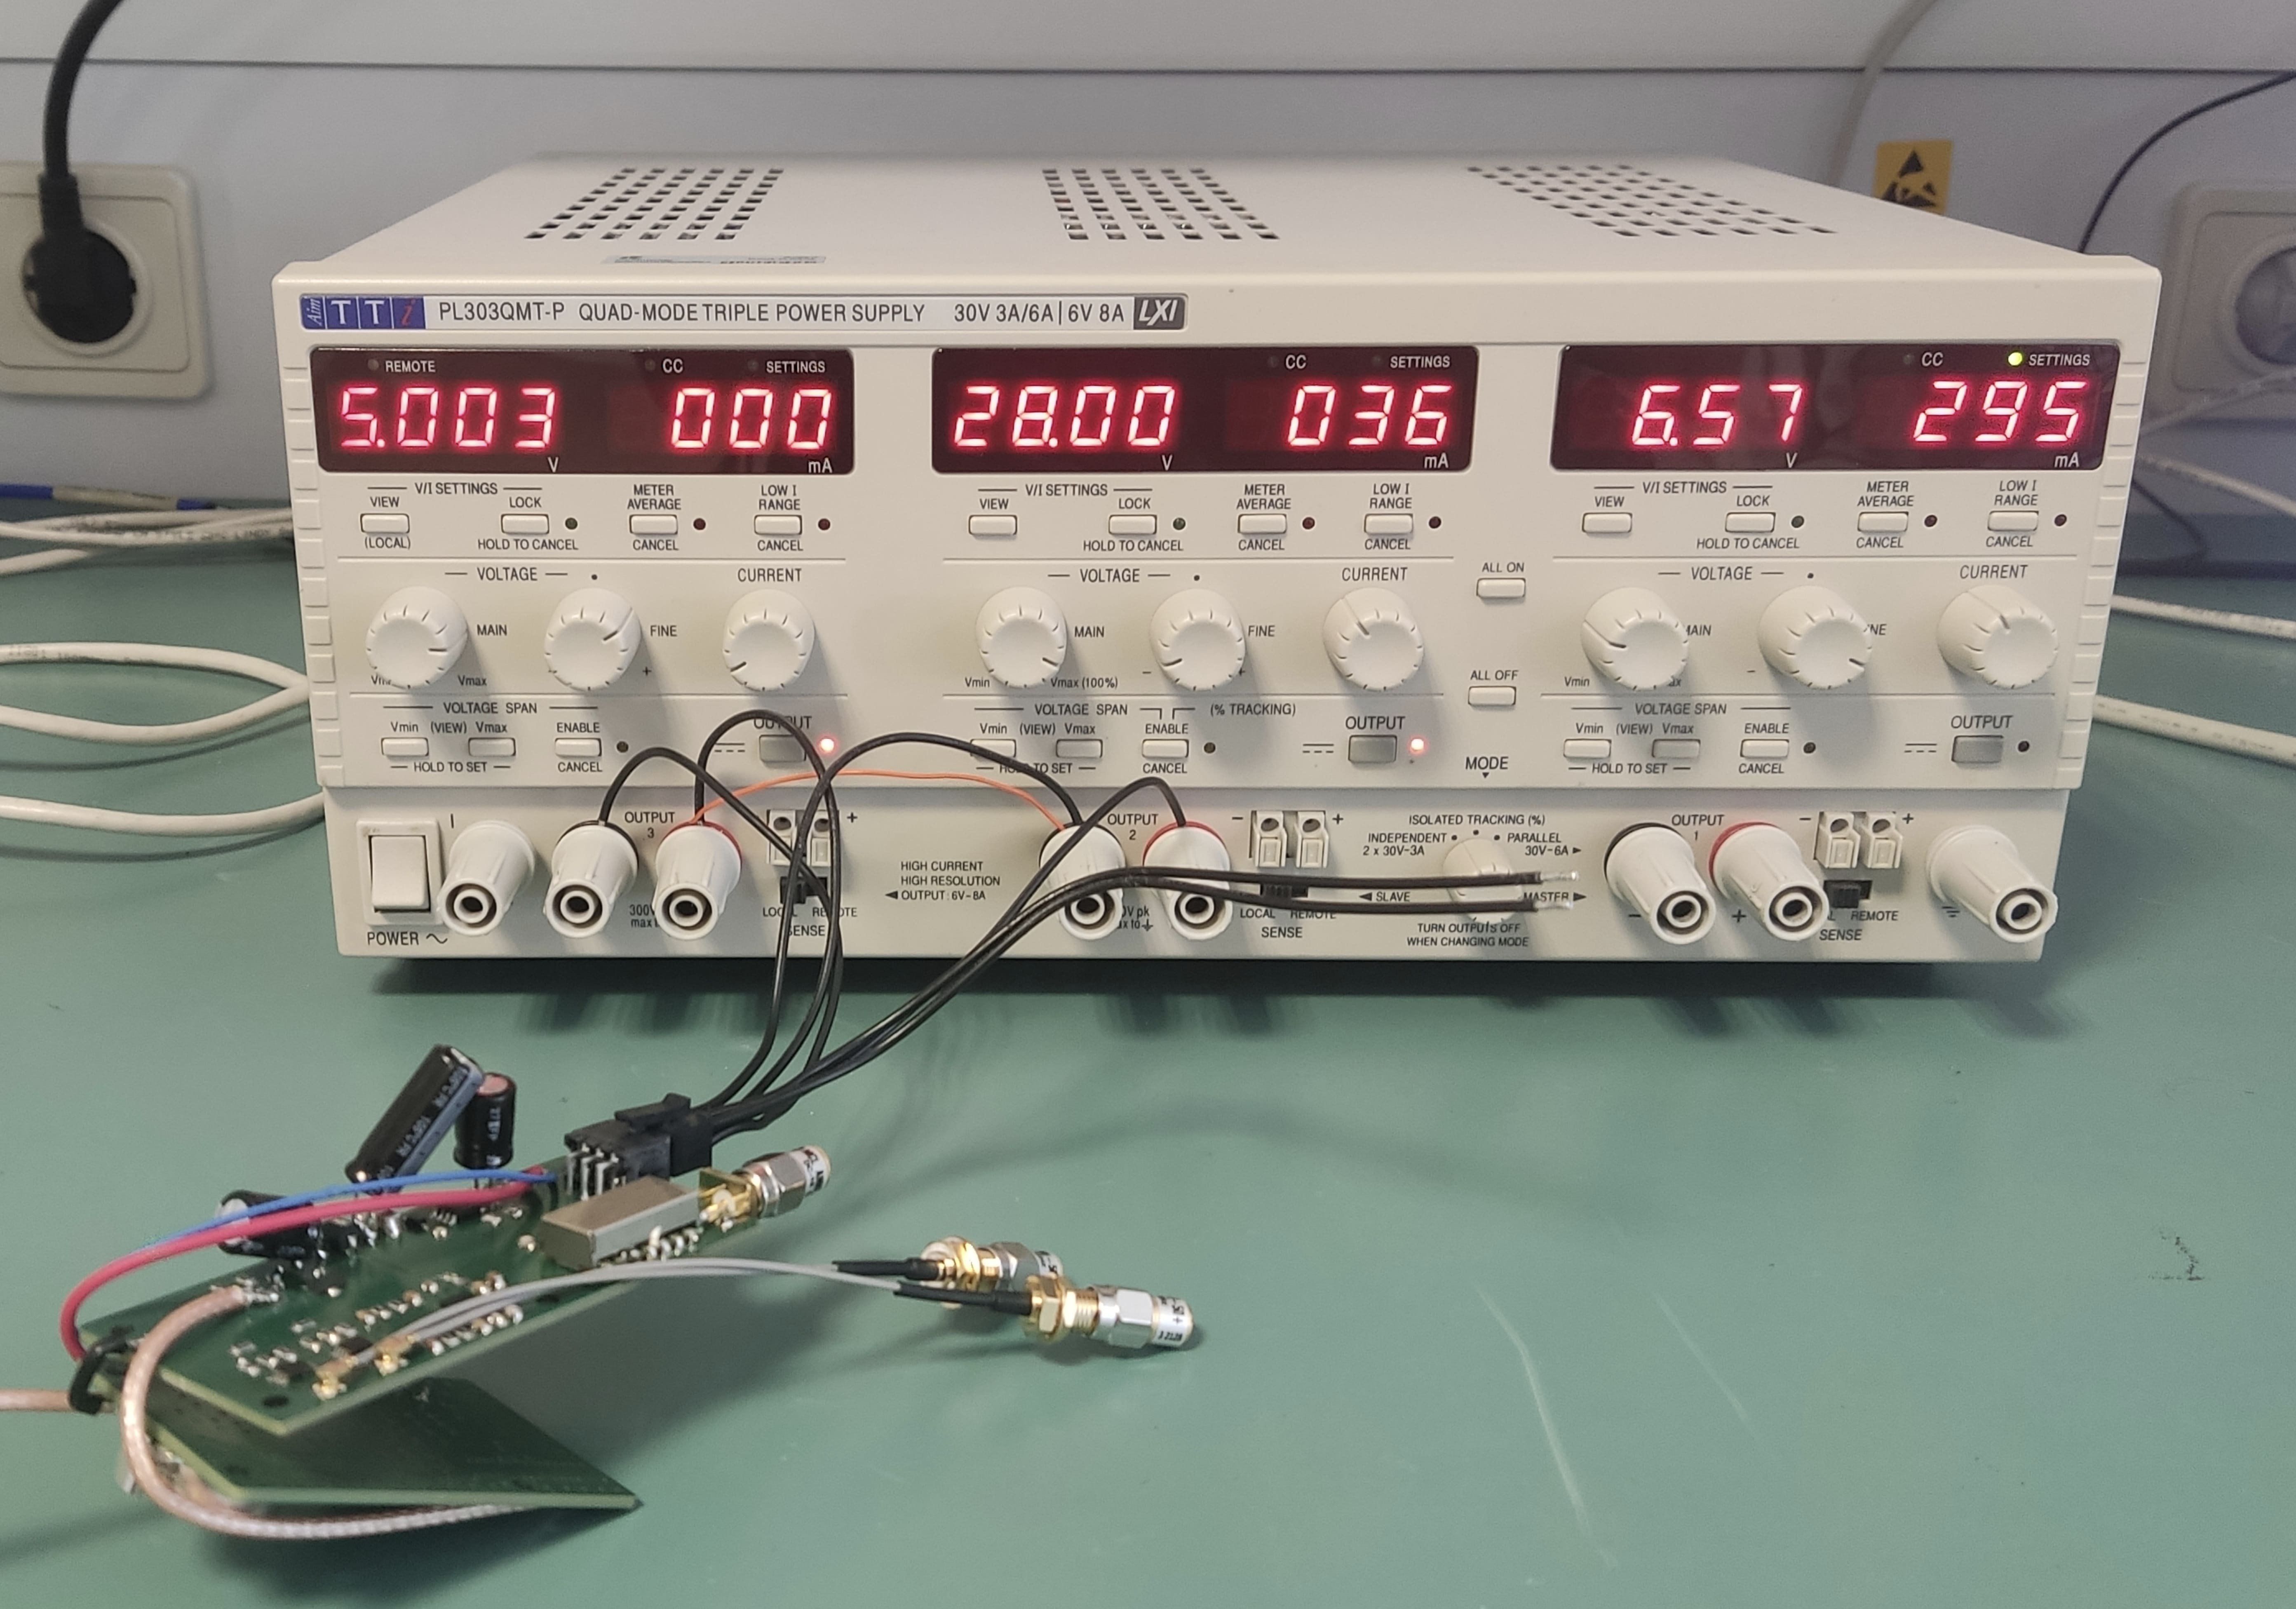
\includegraphics[width=0.7\linewidth]{figs/ch4_psuTesting.jpg}
    \caption{Testing of the Buck Converter Setup}
    \label{fig:ch4_psuTesting.jpg}
\end{figure}


\section{Testing of the Prototype}
\par Following the appropriate biasing protocol mentioned above, we started to record the values of current and $V_{G}$. Figure \ref{fig:ch4_npa1007Pol.png} shows the logged data for this part.

\begin{figure}[H]
    \vspace*{0cm}
    \centering
    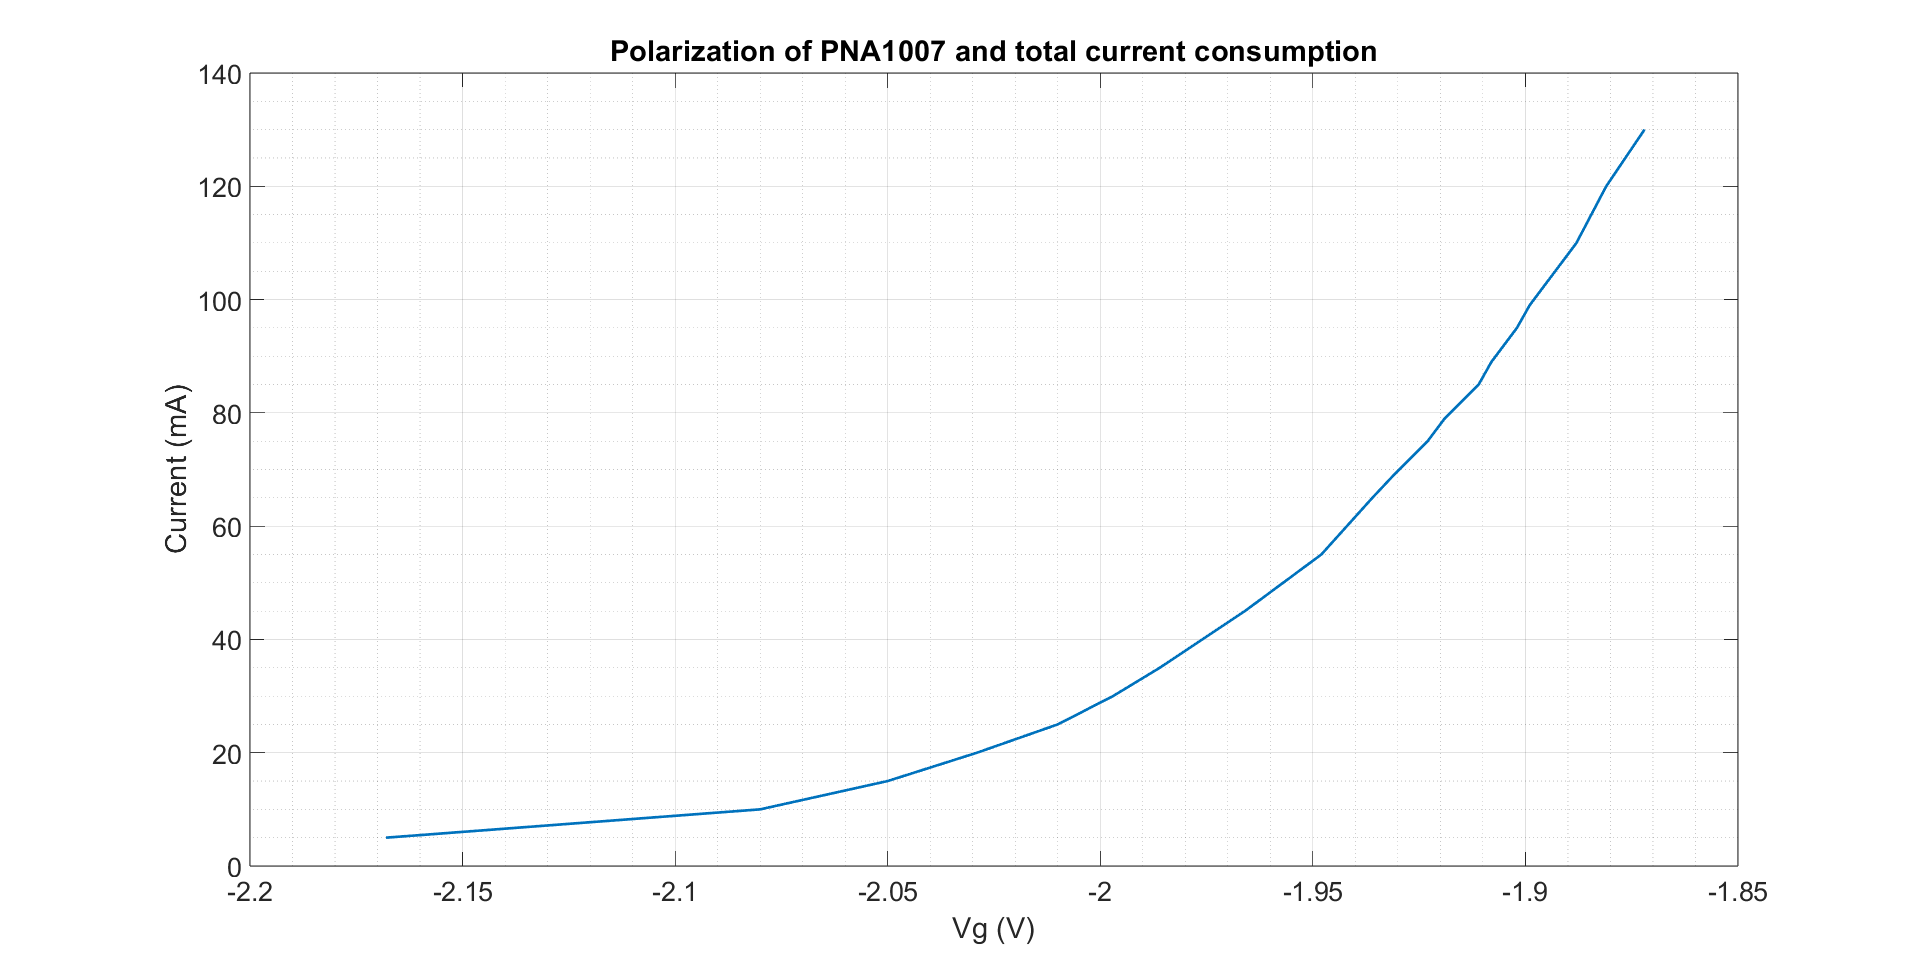
\includegraphics[width=1\linewidth]{figs/ch4_npa1007Pol.png}
    \caption{Testing of the Project Setup}
    \label{fig:ch4_npa1007Pol.png}
\end{figure}

\par We have to note that above a current of $140 \:\si{mA}$ it was noticed that the \ac{pa} would enter thermal runaway. As such, without proper heat dissipation techniques, it is dangerous to allow the circuit to work at certain polarizations without having the current limited in the power supply.

\par In order to test the circuit response to a power input, we tried a setup similar to the one of Figure \ref{fig:ch4_fullSetup.jpg}. The only difference being that the connectors for the \ac{i} and \ac{q} would be terminated by $50\:\si{\Omega}$ loads.

\begin{figure}[H]
    \vspace*{0cm}
    \centering
    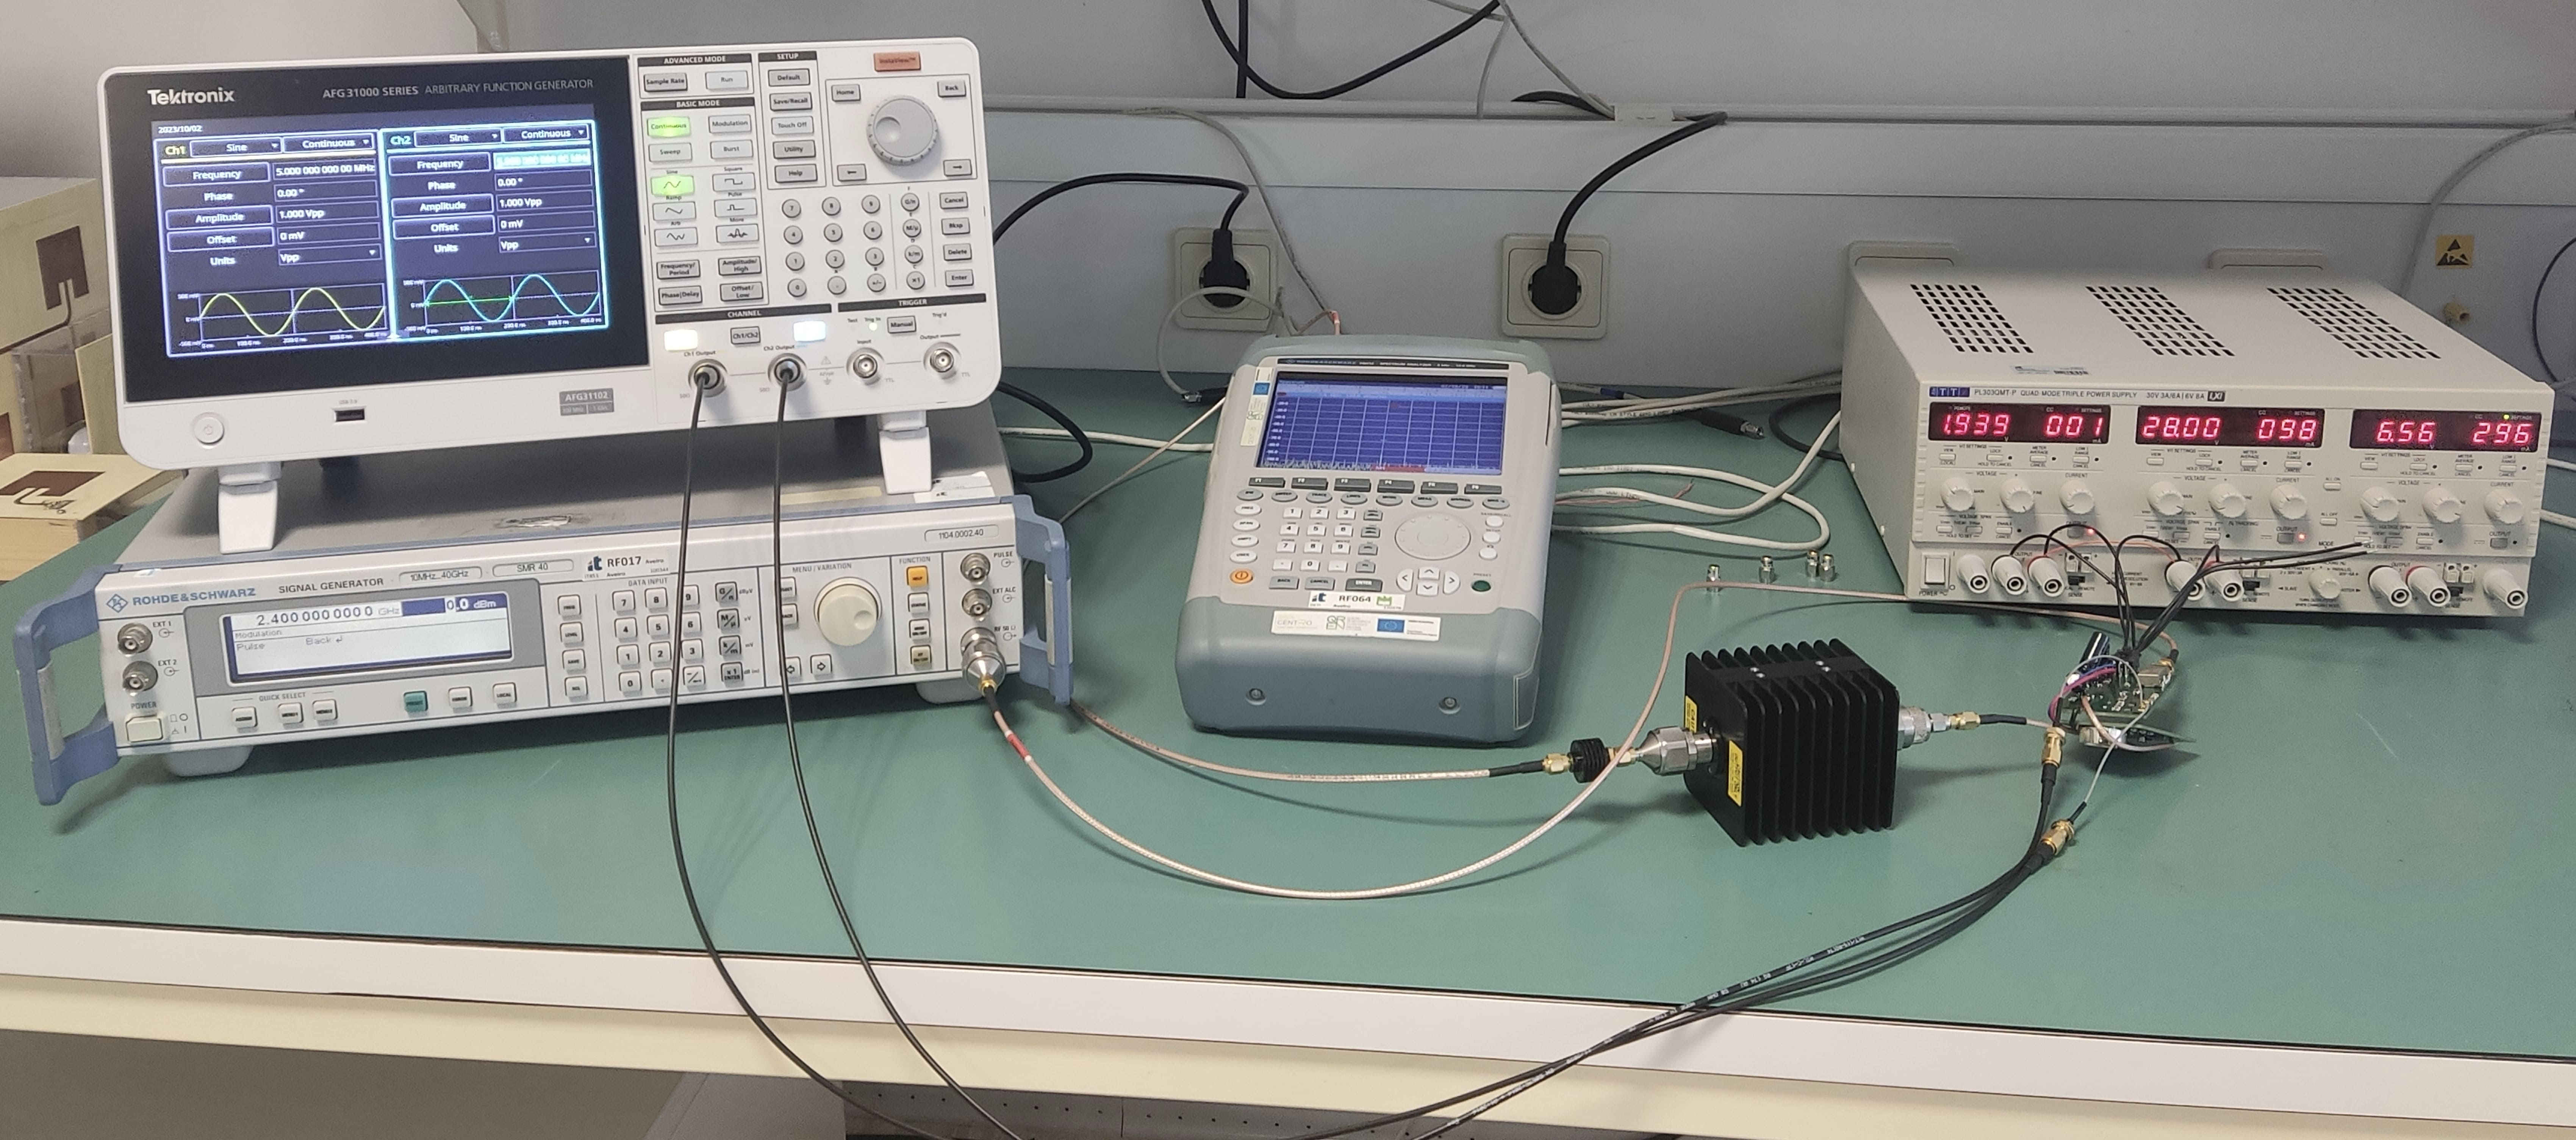
\includegraphics[width=1\linewidth]{figs/ch4_fullSetup.jpg}
    \caption{Testing of the Prototype Setup}
    \label{fig:ch4_fullSetup.jpg}
\end{figure}

\par We proceeded to record the output power delivered by the circuit when supplied with a given input power. The data is presented on Figure \ref{fig:ch4_AMAM.png} in the form of an AM/AM plot.

\begin{figure}[H]
    \vspace*{0cm}
    \centering
    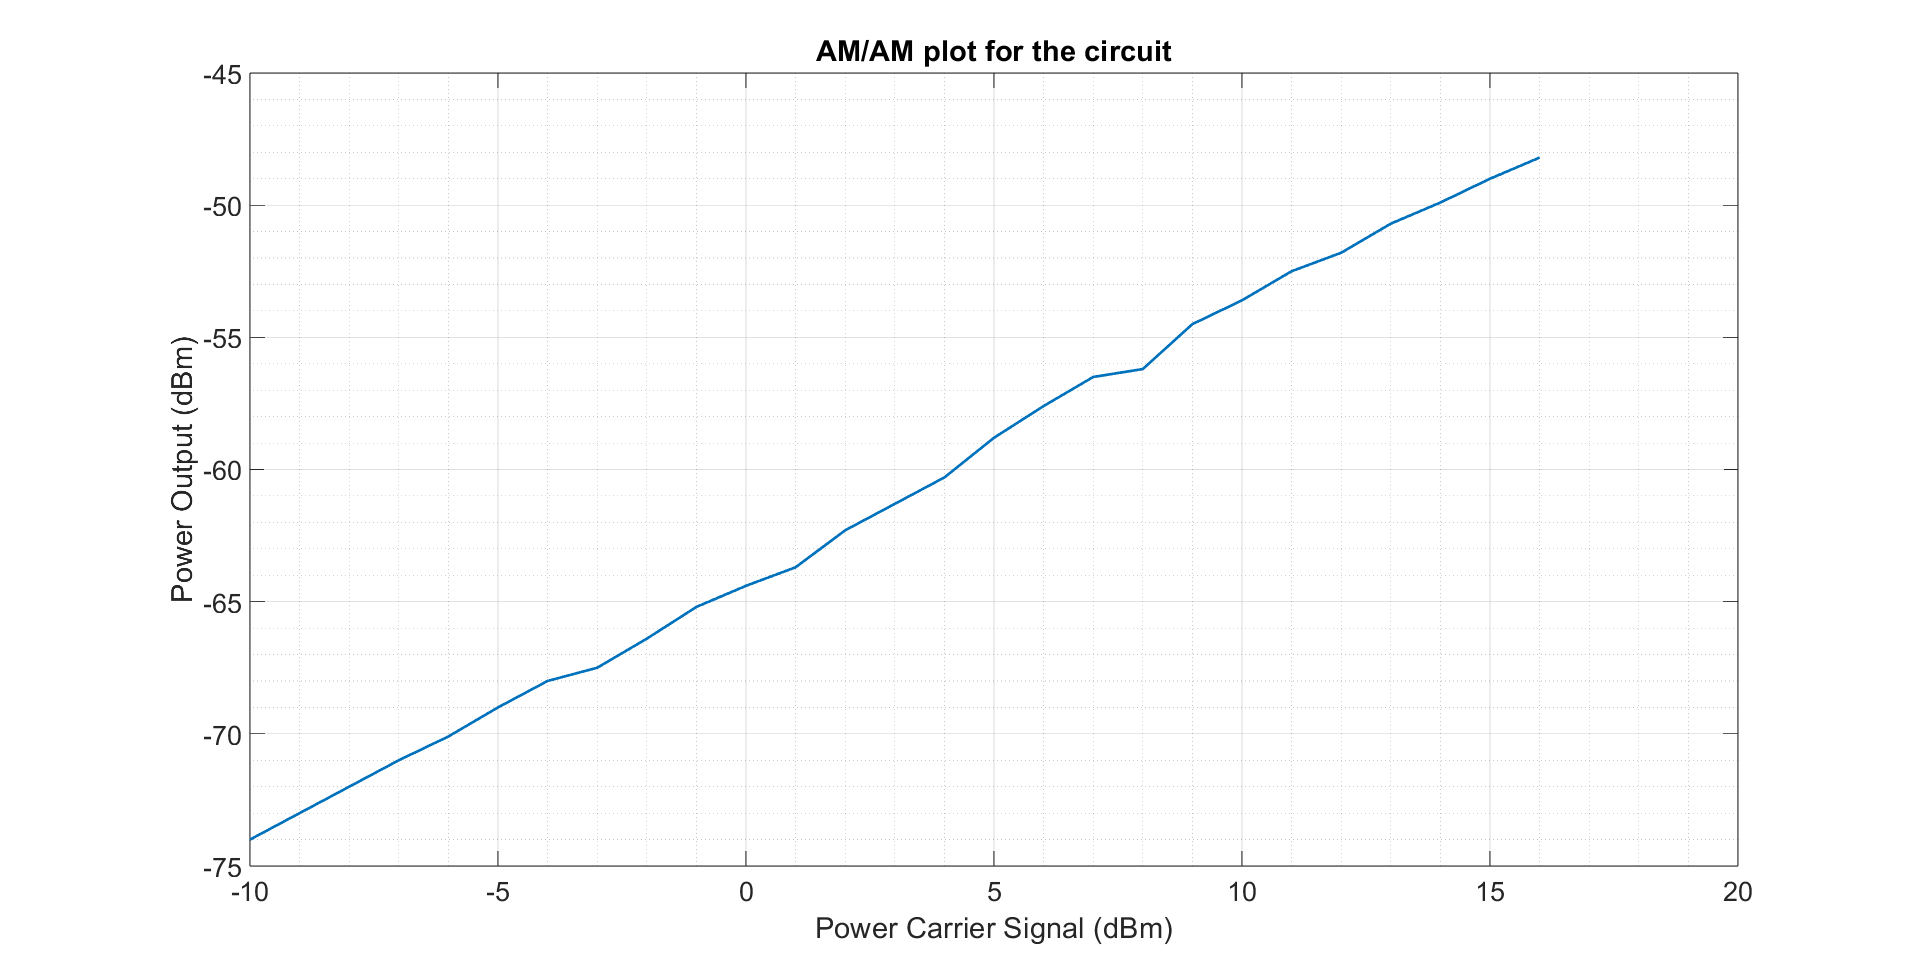
\includegraphics[width=1\linewidth]{figs/ch4_AMAM.png}
    \caption{Testing of the Project Setup using an atenuation of $40 \:\si{dB}$}
    \label{fig:ch4_AMAM.png}
\end{figure}

\par This graph reveals a severe lack of gain on the output signal. Even with a series of attenuators, and the attenuation of the Spectrum Analyzer, the graph shows that the output is delivering an insignificant amount of power. For a maximum input power of $16\:\si{dBm}$, we can see that the output power measured on the Spectrum Analyzer was around $-47\:\si{dBm}$. This output power had been atenuated by $40 \:\si{dB}$, meaning that the actual power at the output of the prototype would be $-7\:\si{dBm}$. There is a possibility that the power being measured at the output of the circuit is nothing more than the leakage power.

\par Next, we tried to repeat the process, only this time with the signals \ac{i} and \ac{q}. We used signals of $2.8\:\si{V}$ of amplitude, centered on $1.4\:\si{V}$ with various frequency values, ranging from $1\:\si{MHz}$ to $2\:\si{0MHz}$. The test setup for the part is as shown in Figure \ref{fig:ch4_fullSetup.jpg}.

\par Unfortunately, there was no change in the circuit response, and we could not verify the presence of any modulation on the output through the Spectrum Analyzer.

\par After suspecting that the problem lay on the quadrature modulator, it was decided to measure the values of the input signals of the modulator, with the inputs terminated on $50\:\si{\Omega}$ loads. Pins 8, 9, 10 and 11 of the modulator read voltages of $[3.292 0.085 2.249 0.247]\:\si{V}$. These values are not consistent with what was expected to be present, showing that the modulator is not working as expected. 

\par We tried to resolder the component in hopes that it would work, but these efforts were in vain. It was then impossible to fully test the circuit. Unfortunately, after the problem was identified and a last resolver attempt was made, there was no more time left to search for another component and make the necessary changes to use another \ac{iq} modulator. As such, solving this issue has to be done in a future prototype.